\begin{figure}[!ht]\centering
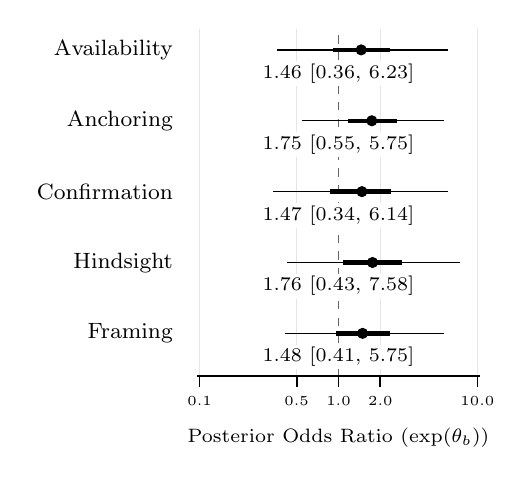
\begin{tikzpicture}[scale=0.9, every node/.style={font=\footnotesize}]
  \draw[gray!20, line width=0.4pt] (-1.96, 0.40) -- (-1.96, 5.30);
  \draw[gray!20, line width=0.4pt] (-0.59, 0.40) -- (-0.59, 5.30);
  \draw[gray!20, line width=0.4pt] (0.59, 0.40) -- (0.59, 5.30);
  \draw[gray!20, line width=0.4pt] (1.96, 0.40) -- (1.96, 5.30);
  \draw[dashed, black!60, line width=0.7pt] (0, 0.40) -- (0, 5.30);
  \node[anchor=east] at (-2.2, 5.00) {Availability};
  \draw[black, line width=0.5pt] (-0.87, 5.00) -- (1.55, 5.00);
  \draw[black, line width=1.6pt] (-0.08, 5.00) -- (0.73, 5.00);
  \filldraw[black] (0.32, 5.00) circle (2pt);
  \node[anchor=north, font=\scriptsize, fill=white, inner sep=1pt] at (0, 4.85) {1.46 [0.36, 6.23]};
  \node[anchor=east] at (-2.2, 4.00) {Anchoring};
  \draw[black, line width=0.5pt] (-0.51, 4.00) -- (1.49, 4.00);
  \draw[black, line width=1.6pt] (0.14, 4.00) -- (0.82, 4.00);
  \filldraw[black] (0.47, 4.00) circle (2pt);
  \node[anchor=north, font=\scriptsize, fill=white, inner sep=1pt] at (0, 3.85) {1.75 [0.55, 5.75]};
  \node[anchor=east] at (-2.2, 3.00) {Confirmation};
  \draw[black, line width=0.5pt] (-0.92, 3.00) -- (1.54, 3.00);
  \draw[black, line width=1.6pt] (-0.12, 3.00) -- (0.74, 3.00);
  \filldraw[black] (0.33, 3.00) circle (2pt);
  \node[anchor=north, font=\scriptsize, fill=white, inner sep=1pt] at (0, 2.85) {1.47 [0.34, 6.14]};
  \node[anchor=east] at (-2.2, 2.00) {Hindsight};
  \draw[black, line width=0.5pt] (-0.72, 2.00) -- (1.72, 2.00);
  \draw[black, line width=1.6pt] (0.07, 2.00) -- (0.90, 2.00);
  \filldraw[black] (0.48, 2.00) circle (2pt);
  \node[anchor=north, font=\scriptsize, fill=white, inner sep=1pt] at (0, 1.85) {1.76 [0.43, 7.58]};
  \node[anchor=east] at (-2.2, 1.00) {Framing};
  \draw[black, line width=0.5pt] (-0.76, 1.00) -- (1.49, 1.00);
  \draw[black, line width=1.6pt] (-0.04, 1.00) -- (0.73, 1.00);
  \filldraw[black] (0.34, 1.00) circle (2pt);
  \node[anchor=north, font=\scriptsize, fill=white, inner sep=1pt] at (0, 0.85) {1.48 [0.41, 5.75]};
  \draw[black, line width=0.6pt] (-2.00, 0.40) -- (2.00, 0.40);
  \foreach \x/\l in {-1.96/0.1, -0.59/0.5, 0/1.0, 0.59/2.0, 1.96/10.0} {
    \draw[black, line width=0.6pt] (\x, 0.40) -- (\x, 0.25);
    \node[below, font=\tiny] at (\x, 0.25) {\l};
  }
  \node[below, font=\scriptsize] at (0, -0.20) {Posterior Odds Ratio ($\exp(\theta_b)$)};
\end{tikzpicture}
\caption{Conditional Manipulation Odds Ratios by Cognitive Bias Family. Reference: Claude Opus 5.5. Thick lines denote 50\% CrI; thin lines denote 95\% CrI.}\label{fig:forest-plot-panel-a}
\end{figure}
